\documentclass{standalone}

\usepackage{pgfplots}
\pgfplotsset{compat=newest}
\usepackage{xcolor}

\begin{document}
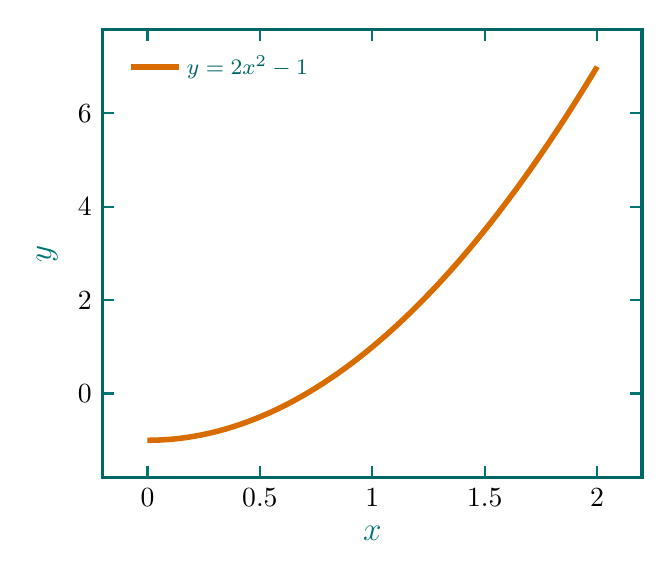
\begin{tikzpicture}
  \begin{axis}[
      xlabel = $x$,
      ylabel = $y$,
      smooth,very thick,
      axis line style = {draw=teal!80!black, very thick, -stealth},
      tick style = {teal!90!black, thick},
      every axis label/.style={font=\large\bfseries, teal!90!black},
      legend style={draw=none, fill=none, font=\bfseries\footnotesize, text=teal!80!black},
      legend pos=north west]

    \addplot[
      color=orange!85!black,
      domain=0:2,
      samples=150,
      line width=2pt
    ]{2*x^2-1};
    \legend{$y = 2x^{2} - 1$}

  \end{axis}
\end{tikzpicture}
\end{document}